\section {Zasada działania}

\subsection {Jak powstaje obraz}

Opracowana przeze mnie implementacja opiera się o pomiar odległości dalmierza od elementów pomieszczcenia dla każdej z możliwości położenia silnika. Innymi słowy silnik obraca się w okół własnej osi a wraz z każdym krokiem wykonuje pomiar odległości.\\

\begin{figure}[h]
    \centering
    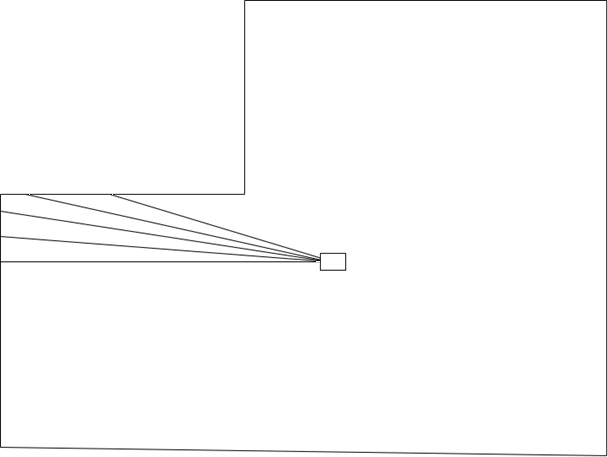
\includegraphics[scale=0.4]{how_it_works_01}
    \caption{Dalmierz na silniku krokowym wykonuje pomiary co jeden krok}
    \label{fig:how_it_works_01}
\end{figure}

Następnie pomierzona odległość zostaje wymnożona przez sinus i cosinus kąta wyznaczonego przez kolejne kroki. Obliczenia te pozwolą nam wyznaczyć wspólrzędne kartezjanskie każdego z mierzonych punktów. Dodać należy że pełny obrót silnika ma 400 gradów, dokonuje więc przeliczenia kąta na wartość radianową.\\

\begin{figure}[h]
    \centering
    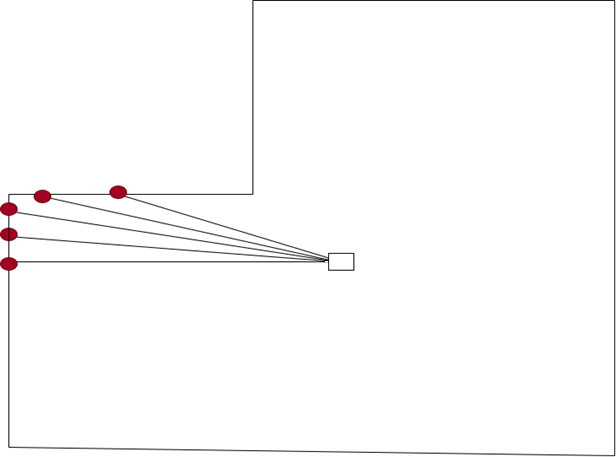
\includegraphics[scale=0.4]{how_it_works_02}
    \caption{Wyznaczane są współrzędne kartezjańskie każdego z punktów}
    \label{fig:how_it_works_02}
\end{figure}

Pełny cykl obrotu silnika daje nam przybliżony obraz całego wewnętrznego obrysu pomieszczenia.\\

\begin{figure}[h]
    \centering
    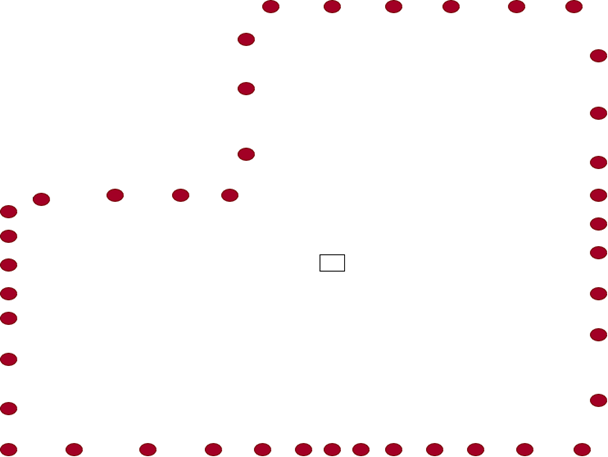
\includegraphics[scale=0.4]{how_it_works_03}
    \caption{Wszystkie wyznaczone punkty dają obrys pomieszczcenia}
    \label{fig:how_it_works_03}
\end{figure}

Na dokładność obrazu składają się: dokładność pomiaru odległości wykonana przez dalmierz, dokładność kąta obrotu silnika krokowego, dokładność obliczeń dla środowiska w którym napisany jest program (Python).\\

Niepewności dla każdego z urządzeń wyznaczone zostały w rozdziale poświęconym specyfikacji sprzętowej projektu.\\